% SECTION ====================================================================================
\section{Dynamische Programmierung}
% ============================================================================================
\vspace{-4pt}
\begin{sectionbox}
\subsection{Idee}\smallskip
\begin{itemize}
    \item Aufteilen eines komplexen Problems in eine vernünftige Anzahl kleinerer Teilprobleme
    \item Die Lösung der Teilprobleme wird zur Lösung des komplexeren Problems verwendet
    \item Identische Teilprobleme werden nur einmal gerechnet
\end{itemize}\smallskip
$\rightarrow$ Wir tauschen Laufzeit gegen Speicherplatz
\end{sectionbox}
\vspace{-4pt}
\begin{sectionbox}
\subsection{Dynamic Programming vs. Divide-And-Conquer}\smallskip
\begin{itemize}
    \item \textbf{Optimale Substruktur}: In beiden Fällen ist das Ursprungsproblem (einfacher) lösbar, indem Lösungen von Teilproblemen herangezogen werden können.
    \item Bei Divide-And-Conquer Algorithmen sind \textbf{Teilprobleme unabhängig}; deren Lösungen werden im Algorithmus nur einmal benötigt.\par
    Beim DP sind Teilprobleme nicht unabhängig. Das Problem hat \textbf{überlappende Teilprobleme}, welche im Algorithmus mehrfach gebraucht werden.
    \item Identische Teilprobleme werden nur einmal gerechnet d.h. \textbf{keine zirkulären Abhängigkeiten zwischen Teilproblemen}
\end{itemize}\smallskip
\end{sectionbox}
\vspace{-4pt}
\begin{sectionbox}
\subsection{Memoization}\smallskip
Memoization (sic) Abspeichern von Zwischenergebnissen.
\begin{itemize}
    \item Bevor ein Teilproblem gelöst wird, wird Existenz eines entsprechenden Zwischenergebnis geprüft
    \item Existiert ein gespeichertes Zwischenergebnis bereits, so wird dieses verwendet.
    \item Andernfalls wird der Algorithmus ausgeführt und das Ergebnis wird entsprechend gespeichert
\end{itemize}\smallskip

\textit{Beispiel Fibonacci}\par
\begin{center}
    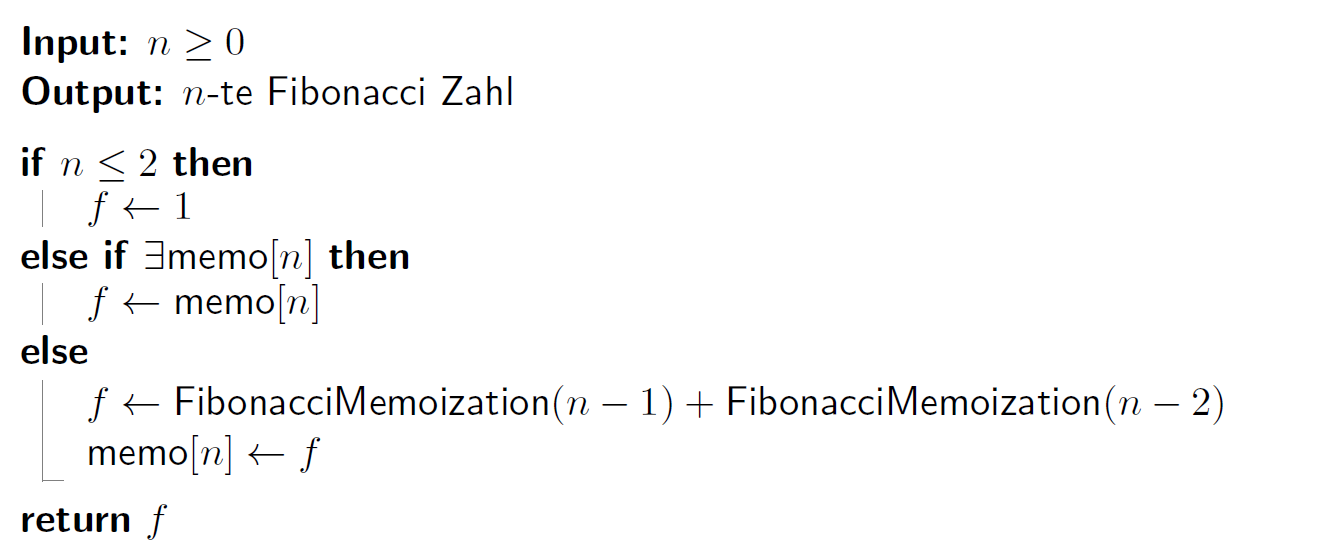
\includegraphics[width = \columnwidth]{../img/memo.png}\par\smallskip
    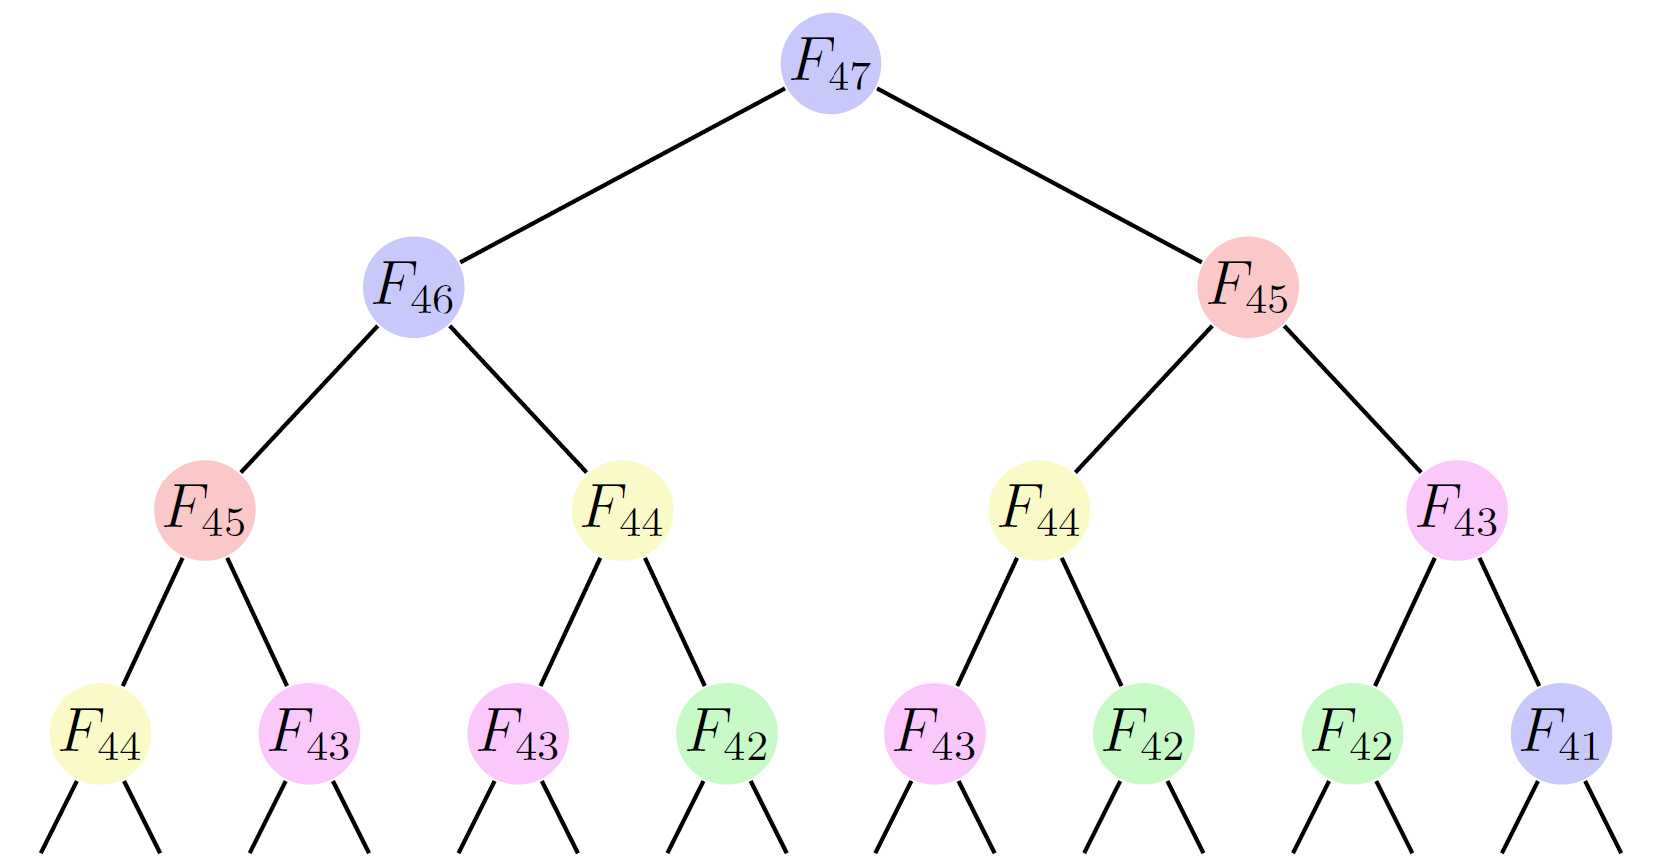
\includegraphics[width = 0.54\columnwidth]{../img/Memo_Fib_schema_vor.png}
    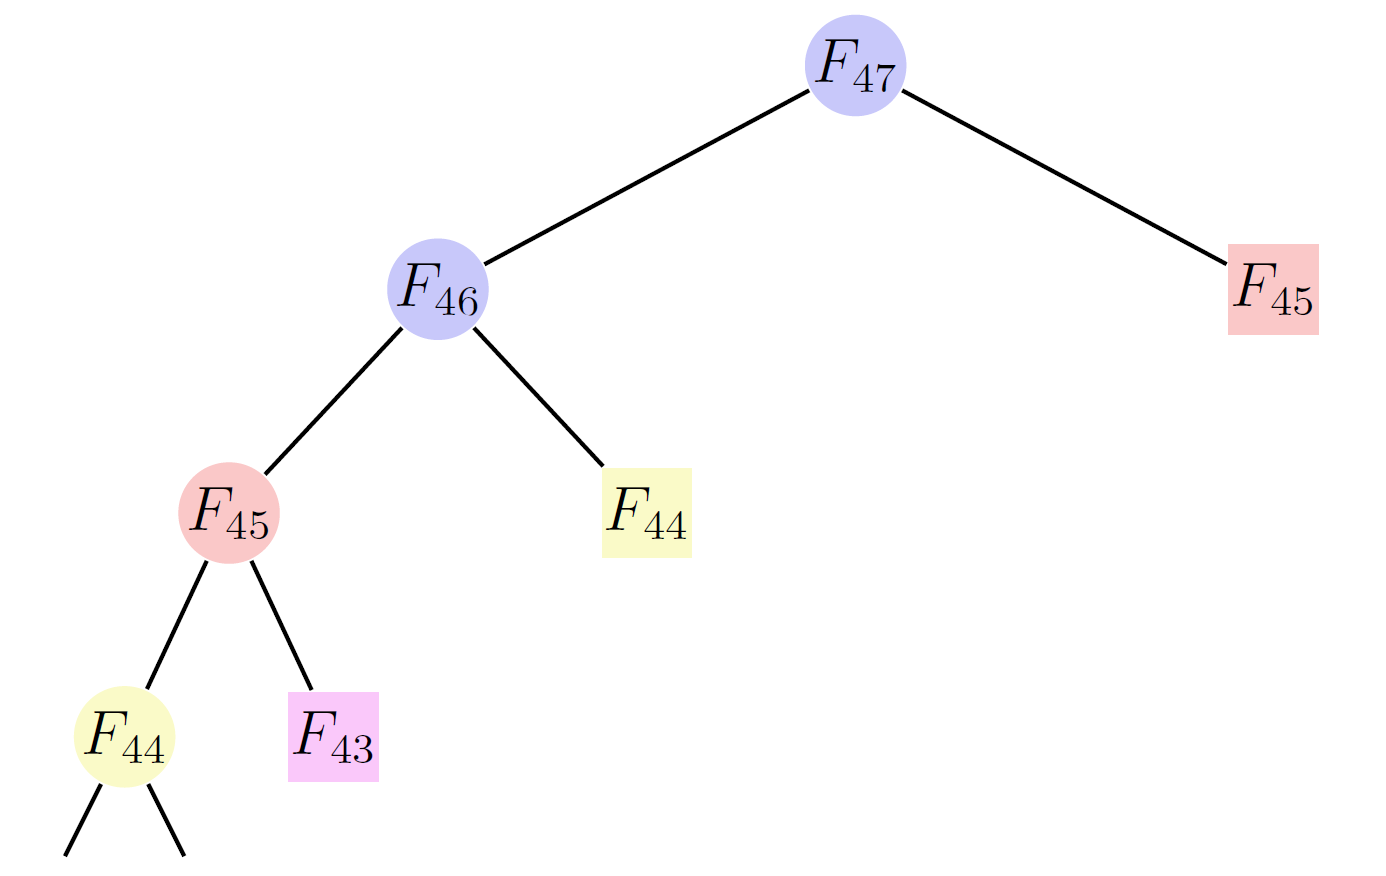
\includegraphics[width = 0.45\columnwidth]{../img/Memo_Fib_schema.png}
\end{center}
$\rightarrow$ Genau hingesehen lösen wir das Problem bottom-up

\end{sectionbox}
\vspace{-4pt}
\begin{sectionbox}
\subsection{Dynamic Programming: Beschreibung am Beispiel}\smallskip

\textit{Beispiel Fibonacci}\par
\begin{center}
    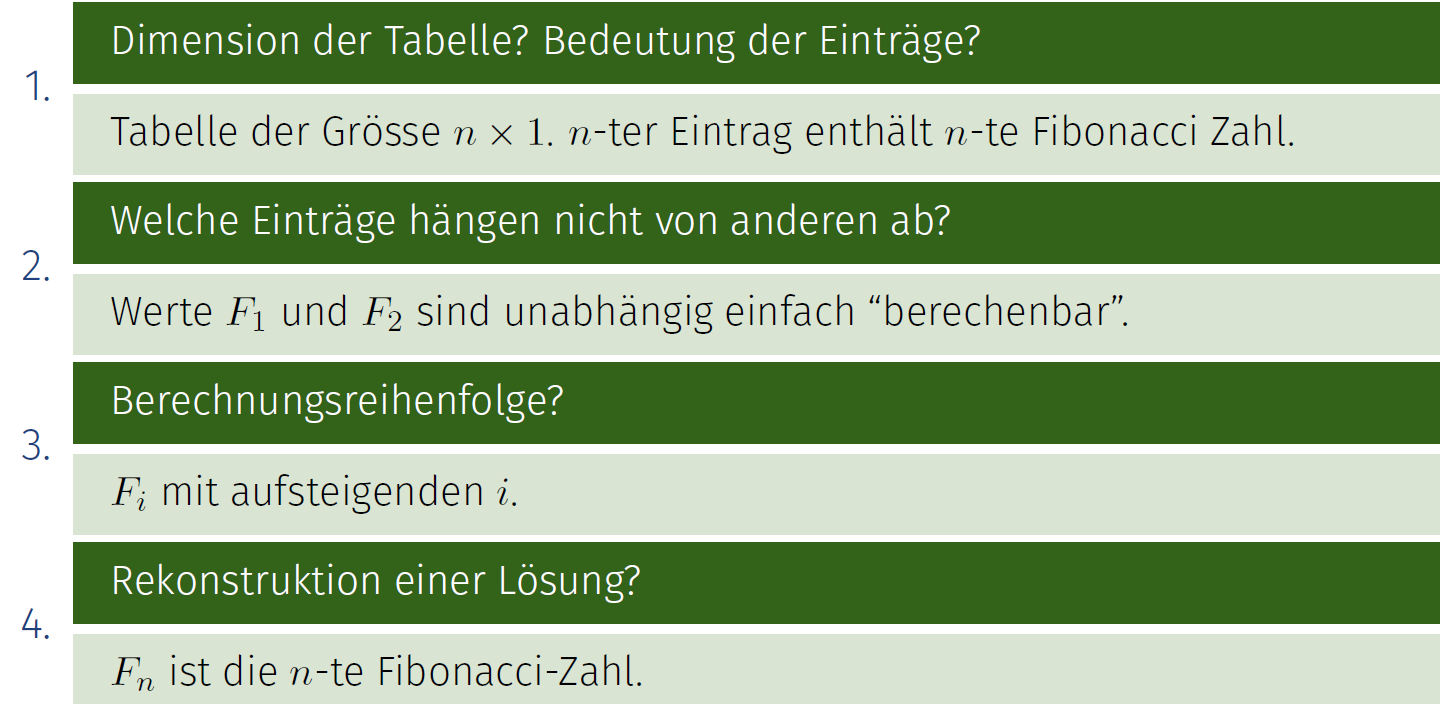
\includegraphics[width = \columnwidth]{../img/DPtable.png}
\end{center}\smallskip

\end{sectionbox}
\vspace{-4pt}
\begin{sectionbox}
\subsection{Wie findet man den DP Algorithmus?}\smallskip
\begin{enumerate}
    \item Genaue Formulierung der gesuchten Lösung
    \item Definiere Teilprobleme (und bestimme deren Anzahl)
    \item Raten / Aufzählen (und bestimme die Laufzeit für das Raten)
    \item Rekursion: verbinde die Teilprobleme
    \item Memoisieren / Tabellieren. Bestimme die Abhängigkeiten der Teilprobleme
    \item Lösung des Problems: \par Laufzeit = Anz. Teilprobleme $\times$ $\frac{\text{Zeit}}{\text{Teilproblem}}$
\end{enumerate}

\end{sectionbox}
\vspace{-4pt}
\begin{sectionbox}
\subsection{Beispiel Kaninchen}\smallskip
Ein Kaninchen sitzt auf Platz (1,1) eines $n \times n$ Gitters. Es kann nur nach Osten oder nach Süden gehen. Auf jedem Wegstück liegt eine Anzahl Rüben. Wie viele Rüben sammelt das Kaninchen maximal ein?\par\smallskip
\begin{center}
    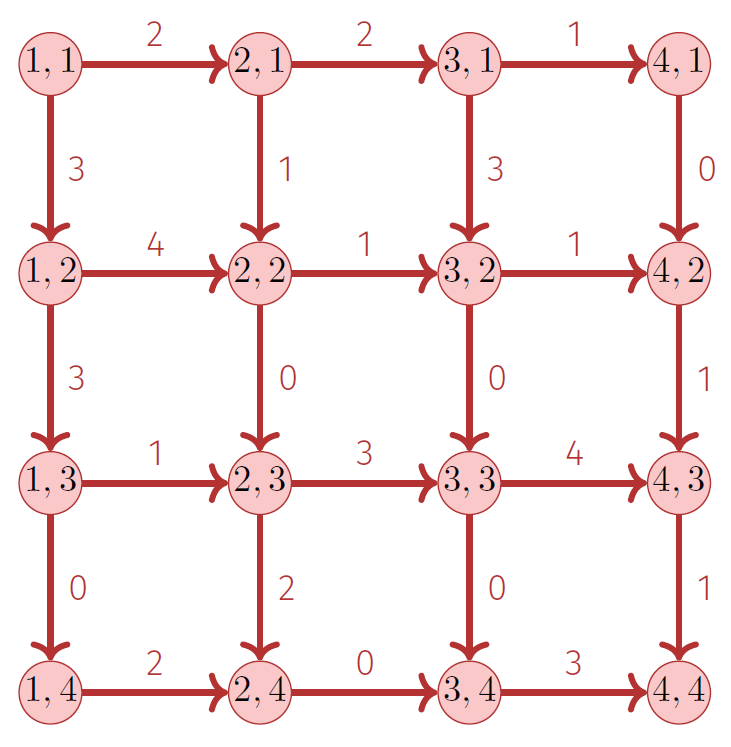
\includegraphics[width = 0.75\columnwidth]{../img/kan1.png}
\end{center}\vspace{7px}
\end{sectionbox}
\vspace{-4pt}
\begin{sectionbox}
\textbf{Rekursion}\par
Gesucht: $T_{0,0}=$ Maximale Anzahl Rüben von (0,0) nach $(n, n)$ Sei $w_{(i, j)-\left(i^{\prime}, j^{\prime}\right)}$ Anzahl Rüben auf Kante von $(i, j)$ nach $\left(i^{\prime}, j^{\prime}\right)$ Rekursion (maximale Anzahl Rüben von $(i, j) \text { nach }(n, n))$\par\smallskip
\begin{center}
    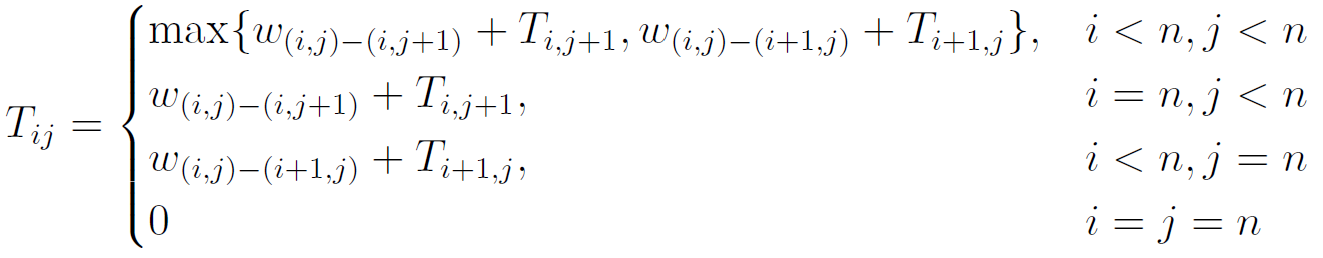
\includegraphics[width = \columnwidth]{../img/kanRek.png}
\end{center}\vspace{7px}
\textbf{Teilabhängigkeitsgraph}\par
\begin{itemize}
    \item Richtung der Abhängigkeiten: Links oben nach rechts unten
    \item Richtung der Berechung: Rechts unten nach links oben
\end{itemize}\vspace{7px}

\end{sectionbox}
\vspace{-4pt}
\begin{sectionbox}
\textbf{Bottom-Up Beschreibung am Beispiel}\par
\begin{center}
    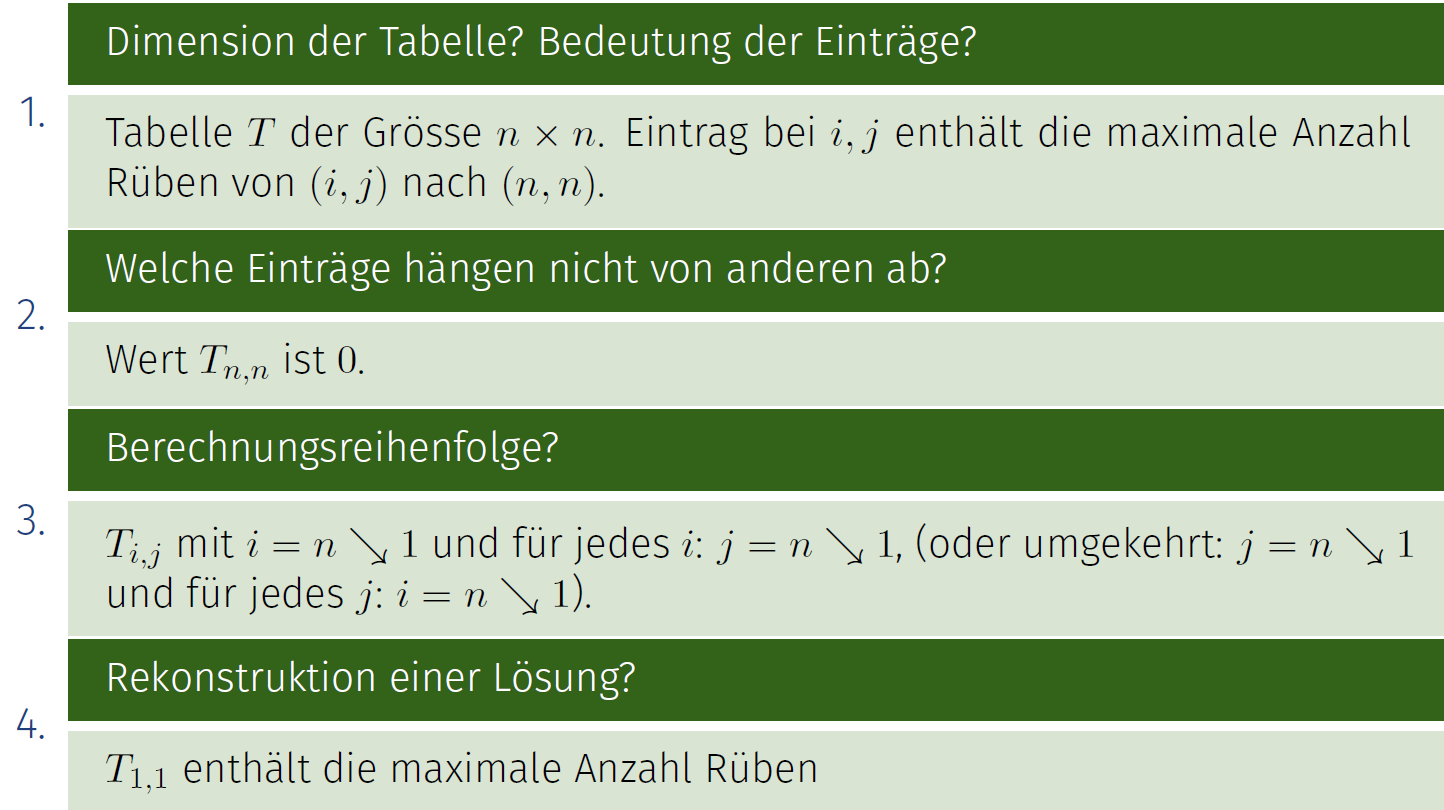
\includegraphics[width = \columnwidth]{../img/kanTable.png}
\end{center}\smallskip

\end{sectionbox}

\vspace{-4pt}
\begin{sectionbox}
\subsection{Die Editierdistanz / Levenshteinabstand}\smallskip
\textbf{Aufgabenstellung}\par
\begin{center}
    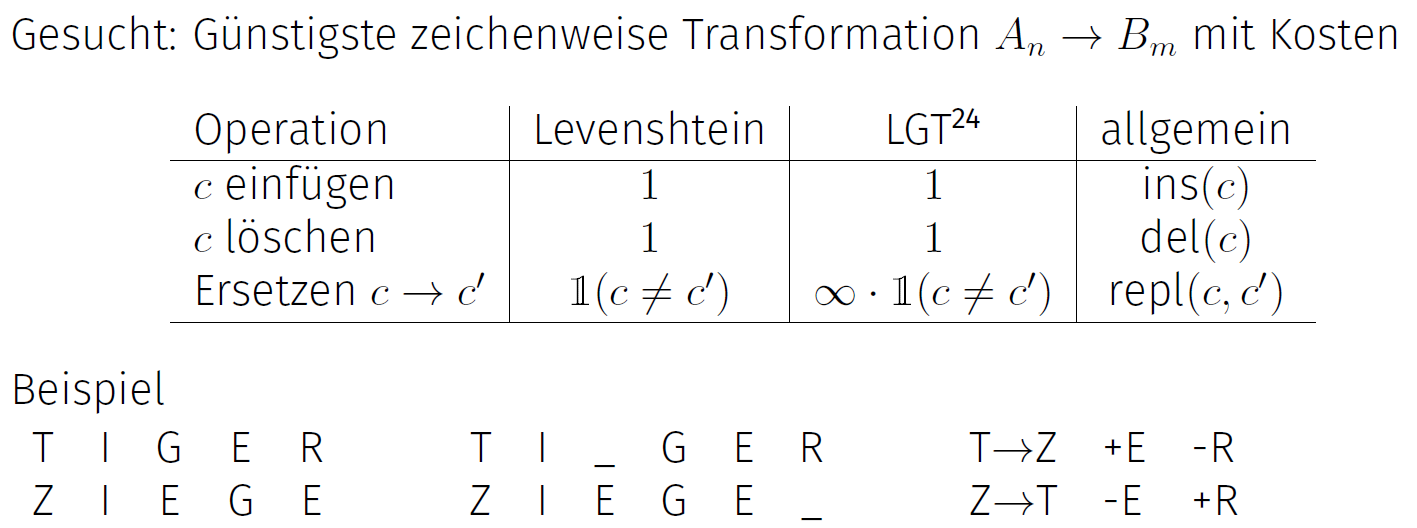
\includegraphics[width = \columnwidth]{../img/ed1.png}
\end{center}\vspace{7px}
\end{sectionbox}
\vspace{-4pt}
\begin{sectionbox}
\textbf{Wie findet man den DP Algorithmus?}\par
\begin{enumerate}
    \item Genaue Formulierung der gesuchten Lösung:
    \par $E(n, m)=$ minimale Anzahl Editieroperationen (ED Kosten) für $a_{1 \ldots n} \rightarrow b_{1 \ldots m}$
    \item Definiere Teilprobleme (und bestimme deren Anzahl):
    \par Teilprobleme $E(i, j)=$ ED von $a_{1 \dots i} . b_{1 \dots j}$ (Anz. $n \cdot m$)
    \item Raten / Aufzählen (und bestimme die Laufzeit für das Raten):
    \par $a_{1 . . i} \rightarrow a_{1 \ldots i-1}(\text { löschen })$
    $a_{1 . . i} \rightarrow a_{1 \ldots i} b_{j}$ (einfügen)
    $a_{1 . . i} \rightarrow a_{1 \ldots i-1} b_{j}$ (ersetzen)
    \item Rekursion: verbinde die Teilprobleme:
    \par \begin{center}
        $E(i, j)=\min \left\{\begin{array}{l}\operatorname{del}\left(a_{i}\right)+E(i-1, j) \\ \operatorname{ins}\left(b_{j}\right)+E(i, j-1) \\ \operatorname{repl}\left(a_{i}, b_{j}\right)+E(i-1, j-1)\end{array}\right.$
    \end{center}
    \item Memoisieren / Tabellieren. Bestimme die Abhängigkeiten der Teilprobleme:
    \par \begin{center}
        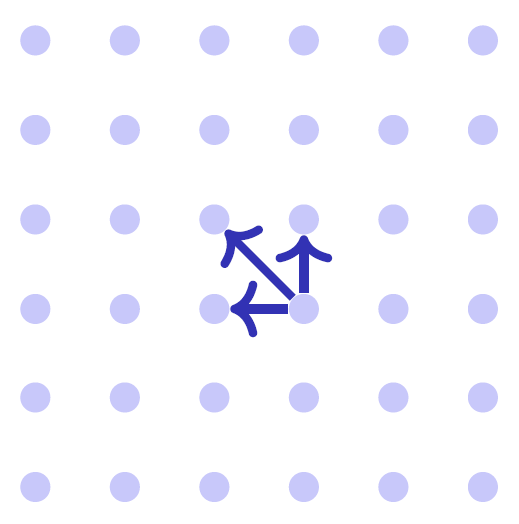
\includegraphics[width=0.4\columnwidth]{../img/Lst_Abh.png}
    \end{center}
    \par Berechnung von links oben nach rechts unten. Zeilen- oder Spaltenweise.
    \item Lösung des Problems: Lösung steht in $E(n, m)$
\end{enumerate}\vspace{7px}
\end{sectionbox}
\vspace{-4pt}
\begin{sectionbox}
\textbf{Bottom-Up Beschreibung}\par
\begin{center}
    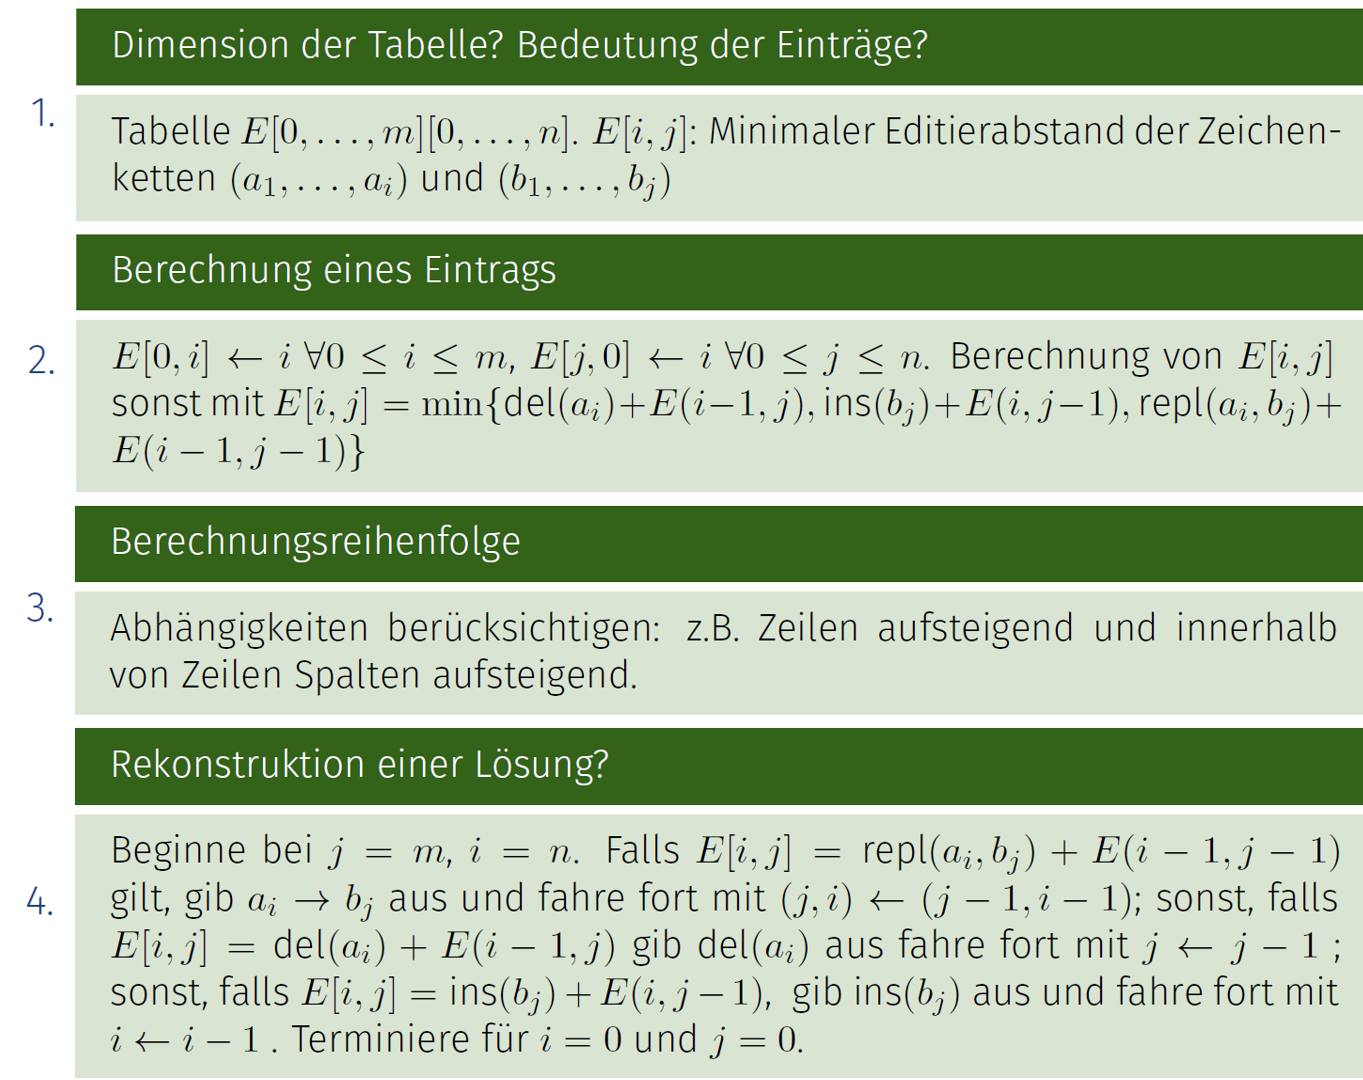
\includegraphics[width = \columnwidth]{../img/edTable.png}
\end{center}\smallskip

\textbf{Analyse}\par
Anzahl Tabelleneinträge: $(m+1) \cdot (n+1)$\par
Laufzeit: $\mathcal{O}(m \cdot n)$\smallskip
\end{sectionbox}
\vspace{-4pt}
\begin{sectionbox}
\subsection{Kürzeste Wege: DP Ansatz (Bellman)}\smallskip
Induktion über Anzahl Kanten $d_{s}[i, v]$: Kürzeste Weglänge von $s$ nach $v$ über maximal $i$ Kanten.\par\vspace{-3px}
\begin{equation*}
\begin{array}{l}
d_{s}[i, v]=\min \left\{\begin{array}{l} d_{s}[i-1, v] \\ \min _{(u, v) \in E}\left(d_{s}[i-1, u]+c(u, v)\right)\end{array}\right. \\
d_{s}[0, s]=0, \underbrace{d_{s}[0, v]=\infty \forall v \neq s}_{\text{Zyklus}}
\end{array}
\end{equation*}\par\smallskip
\begin{center}
    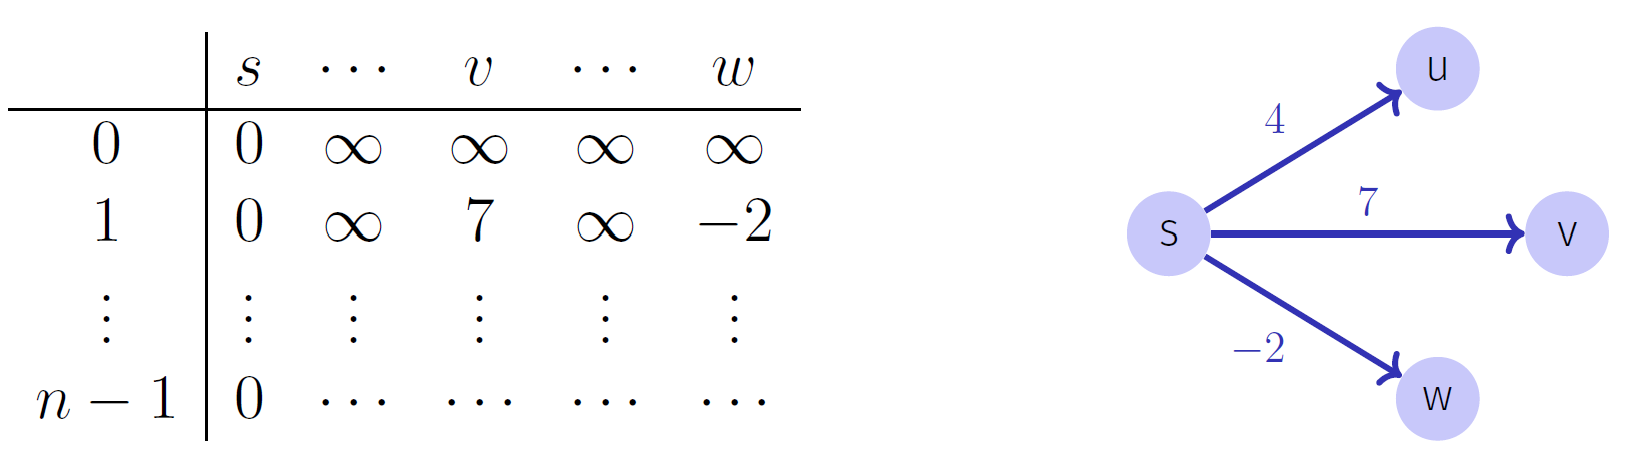
\includegraphics[width = 0.9\columnwidth]{../img/BellFordSym.png}
\end{center}\smallskip
Algorithmus: Iteriere über letzte Zeile bis die Relaxationsschritte keine Änderung mehr ergeben, maximal aber $n − 1$ mal. Wenn dann noch Änderungen, dann gibt es keinen kürzesten Pfad.\par\vspace{7px}

\textbf{Bellmann-Ford(G,s)}\par
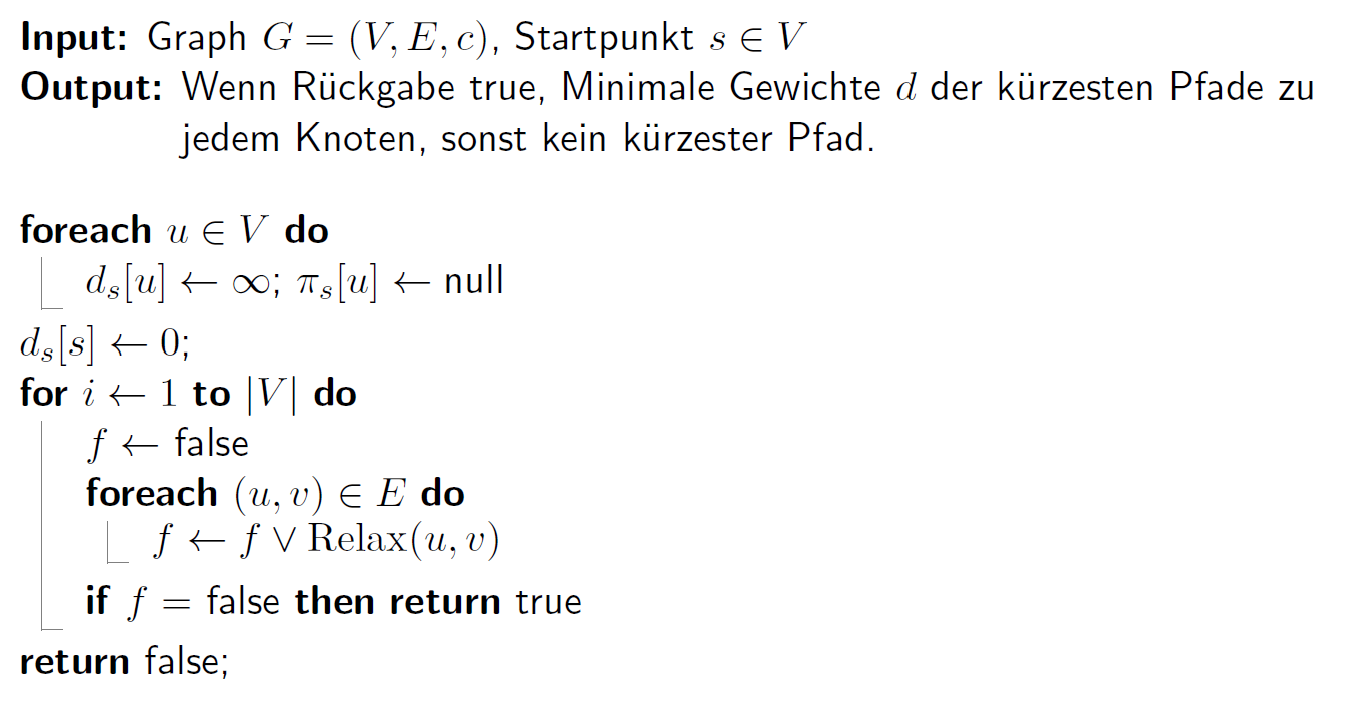
\includegraphics[width = \columnwidth]{../img/BellFord.png}\smallskip

\textbf{Analyse}\par
Laufzeit: $\mathcal{O}(|V| \cdot |E|)$\par
Speicherplatz: $\mathcal{O}(|V|^2)$ $\leadsto$ eigentlich sogar $\mathcal{O}(|V|)$, da nur immer die letzte Zeile abgespeichert werden muss.\smallskip
\end{sectionbox}